% Commands
% !TEX encoding = UTF-8 Unicode
% !TEX TS-program = pdflatex

% Document class
\documentclass[%
    corpo=12pt,
    twoside,
    %    stile=classica,
    oldstyle,
    %    autoretitolo,
    tipotesi=magistrale,
    greek,
    evenboxes,
]{toptesi}
\usepackage[utf8]{inputenc}
\usepackage[T1]{fontenc} % font encoding
\usepackage{lmodern} % font
\pdfminorversion=5

% Table of contents
\usepackage[nottoc,notlof,notlot]{tocbibind} % including references
\setcounter{tocdepth}{2} % depth
\setcounter{secnumdepth}{3} % section numbering depth

% Front page
\renewcommand\IDlabel{\\\quad Student ID:\xspace}

% Miscellaneous
% \usepackage{fullpage} % different margins
\usepackage[hidelinks]{hyperref} % links
% \hypersetup{
%     pdfpagemode={UseOutlines},
%     bookmarksopen,
%     pdfstartview={FitH},
%     colorlinks,
%     linkcolor={blue},
%     citecolor={blue},
%     urlcolor={blue}
% }
\usepackage[binary-units=true]{siunitx} % MB, GB, etc.
\usepackage{pdfpages} % import PDFs
\usepackage{verbatim} % multi-line comments

% Checkmarks and x-marks
\usepackage{amssymb}
\usepackage{pifont}
\definecolor{green}{RGB}{0,176,80}
\newcommand{\cmark}{{\color{green}\textbf{\ding{51}}} }
\definecolor{red}{RGB}{222,0,0}
\newcommand{\xmark}{{\color{red}\textbf{\ding{55}}} }

% Adding a dot at the end of paragraph titles
\let\originalparagraph\paragraph
\renewcommand{\paragraph}[2][.]{\originalparagraph{#2#1}}

% Glossaries and acronyms
\usepackage[acronym,toc]{glossaries} % package
% General
\newacronym{api}{API}{Application Programming Interface}
\newacronym{rm}{RM}{Resource Manager}
\newacronym{vm}{VM}{Virtual Machine}
\newacronym{inp}{INP}{In-Network Processing}
\newacronym{nfv}{NFV}{Network Function Virtualization}
\newacronym{sdn}{SDN}{Software Defined Networking}
\newacronym{voc}{VOC}{Virtual Oversubscribed Cluster}
\newacronym{tor}{ToR}{Top of Rack}
\newacronym{mpi}{MPI}{Message Passing Interface}
\newacronym{hpc}{HPC}{High Performance Computing}

% CloudMirror
\newacronym{tag}{TAG}{Tenant Application Graph}

% SHArP
\newacronym{an}{AN}{Aggregation Node}
\newacronym{am}{AM}{Aggregation Manager}
\newacronym{tca}{TCA}{Target Channel Adapter}
\newacronym{qp}{QP}{Queue Pair} % acronyms
\paragraph{Data center architecture} \label{dc_architecture}
% Data center fat-tree
    % Also network resources
        % Uniform compute units (CU) and properties
This simulator emulates \glspl{resource:physical:switch} besides \glslink{resource:physical:server}{server ones}.
It can support any kind of data center network architecture.
Specifically, a \textit{fat-tree} has been used for this evaluation, which is a very common topology for data centers to use. An example of a fat-tree topology is depicted in \autoref{fig:fattree}.
\begin{figure}[!htb]
    \centering
    \usebox{\fattree}
    \caption{A fat-tree topology with 4 \textit{pods}}
    \label{fig:fattree}
\end{figure}

This fat-tree has three layers of \glslink{resource:physical:switch}{switches}: \textit{core}, \textit{aggregation} and the last one which is usually called \textit{edge}, \textit{layer}, \textit{access} or just simply \gls{tor} \glslink{resource:physical:switch}{switches}.
Being $k$ the number of \textit{pods} in the topology, a fat-tree contains $(k/2)^2$ core \glslink{resource:physical:switch}{switches}, $k^2/2$ aggregation \glslink{resource:physical:switch}{switches}, $k^2/2$ \gls{tor} \glslink{resource:physical:switch}{switches}, and supports up to $k^3/4$ \glslink{resource:physical:server}{servers}.
Being then $5k^2/4$ the total amount of \glslink{resource:physical:switch}{switches} in a fat-tree, \glslink{resource:physical:server}{servers} become more abundant when $k>5$.

\paragraph{\Glspl{resource:physical:switch}} \label{simulator_switch_resources}
\glsreset{cu}
For the sake of simplicity, \glslink{resource:physical:switch}{physical switches} have a single numerical dimension called \gls{cu}.
This assumption does not affect this evaluation's results and it makes the scheduling algorithm a bit simpler.
Increasing the number of \glslink{resource:physical:switch}{switch} dimensions is trivial since the simulator already supports multiple dimensions for \glslink{resource:physical:server}{servers}, namely CPU and memory.
\Glspl{resource:logical:edge} have been ignored to simplify the placement algorithm.

\glslink{resource:physical:switch}{Switches} are also characterized by a \textit{property map}, that ultimately suggests which kinds of \gls{inp} solutions they are able to run.
In this evaluation, properties and \gls{inp} solutions coincide (e.g., \glslink{resource:physical:switch}{switch} $A$ supports \gls{inp} solutions $X$, $Y$, and $Z$), but these properties might be more appropriately extended to any other kind of hardware property that distinguish \glslink{resource:physical:switch}{switches} in the data center (e.g., CPU architecture, supported data plane programming language, etc.).
In general, a switch task requesting for property $P$ will only be allocated on a \glslink{resource:physical:switch}{switch} if it supports that same property $P$. % resources glossary
\makenoidxglossaries % computing the glossary and acronyms list

% In-line lists
\usepackage[inline]{enumitem}
\newlist{mylist}{enumerate*}{1}
\setlist[mylist]{label=(\roman*)}

% References sections
\renewcommand{\sectionautorefname}{\S}
\renewcommand{\subsectionautorefname}{\S}
\renewcommand{\subsubsectionautorefname}{\S}
\renewcommand\bibname{References}

% Capitalized references
\usepackage{cleveref}

% Footnotes with symbols
\usepackage[symbol]{footmisc}
\renewcommand{\thefootnote}{\fnsymbol{footnote}}

% Blank pages
\usepackage{afterpage}
\newcommand\blankpage{%
    \null
    \thispagestyle{empty}%
    \addtocounter{page}{-1}%
    \newpage
}

% Comments
\newcommand\pnote[1]{\textit{\textcolor{blue}{[p@]: #1}}}
\newcommand\ma[1]{\textit{\textcolor{purple}{[marcel]: #1}}}
\newcommand\lin[1]{\textit{\textcolor{green!55!blue}{[lin]: #1}}}
\newcommand\marco[1]{\textit{\textcolor{red}{[marco]: #1}}}
\newcommand\fulvio[1]{\textit{\textcolor{orange}{[fulvio]: #1}}}

% Document start
\begin{document}
\noindent

% This is the thesis summary document
\newcommand*\THESISSUMMARY{}

% Title
% \begin{titlepage}
%     \begin{center}
%         \vspace*{7cm}
 
%         \Huge
%         \textbf{Data center resource management for in-network processing}
 
%         \vspace{1cm}
        
%         \huge
%         Marco Micera
 
%         \vfill
 
%         \LARGE
%         \textit{Politecnico di Torino, TU Darmstadt}
%     \end{center}
% \end{titlepage}

\begin{ThesisTitlePage}
    % Per cambiare la dicitura sopra la lista dei laureandi decommentare
    % la riga seguente, cambiando le 4 parole in modo consistente
    %
    \TitoloListaCandidati{Studente,Studenti,Studentessa,Studentesse}
    %
    \ateneo{Politecnico di Torino, TU Darmstadt}
    %
    % Non tutte le università hanno un nome proprio
    % \nomeateneo{DAUIN - Department of Control and Computer Engineering, DSP - Distributed Systems Programming Group}
    %
    \struttura[III]{Matematica, Fisica e~Scienze Naturali}
    %\Materia{Remote sensing}
    \titolo{Data center resource management for in-network processing}% per la laurea quinquennale e il dottorato
    % \sottotitolo{Metodo dei satelliti medicei}% per la laurea quinquennale e il dottorato
    %
    %%%%%%% Corso degli studi
    \corsodilaurea{Computer Engineering}% per la laurea
    
    %%%%%%% L'eventuale numero di matricola va fra parentesi quadre
    %\show\Candidato
    \def\Candidato{Candidate}
    %\show\Candidato
    \candidato{Marco \textsc{Micera}}[253157] 
    %\secondocandidato{Evangelista \textsc{Torricelli}}[123457]
    
    %%%%%%% Relatori o supervisori
    %
    \def\Relatori{Supervisors}
        \relatore{Prof. Fulvio Risso}
        \secondorelatore{Prof. Patrick Eugster}
        \terzorelatore{M.Sc. Marcel Bl{\"o}cher}
    % 
    %%%%%%% Per mettere altri relatori consultare toptesi-it.pdf
    
    %%%%%%% Tutore
    % \tutoreaziendale{dott.\ ing.\ Giovanni Giacosa}
    % \NomeTutoreAziendale{Supervisore aziendale\\Centro Ricerche FIAT}
    
    %%%%%%% Seduta dell'esame
    %\sedutadilaurea{Agosto 1615}
    %%%%%%%% oppure:
    \sedutadilaurea{April, 2020}% 
    
    %%%%%%% Logo della sede
    % \logosede{logodue}% 
    \end{ThesisTitlePage}


%
% Compliant to the thesis summary needed by the ICM/ETF board secretary
%
% 1. title, graduand name, supervisors names
% 2. thesis purpose and brief description of the research area
% 3. personal contribution and results obtained
%
% 3 pages max
%

% Sections
\section{Info}
\textbf{Title}: Data center resource management for in-network processing\\
\textbf{Graduand name}: Marco Micera\\
\textbf{Supervisors}: Prof. Fulvio Risso \footnote[2]{\label{polito} Computer Networks Group, Politecnico di Torino, Italy}, Prof. Patrick Eugster \footnote[3]{\label{tuda} Distributed Systems Programming Group, Technische Universit{\"a}t Darmstadt, Germany}, M.Sc. Marcel Bl{\"o}cher \footref{tuda}\\
\textbf{Research areas}: cloud computing, distributed systems, data centers

\section{Thesis purpose}
Nowadays there exist several \gls{inp} solutions that allow tenants to improve their application performance in terms of different metrics: \textsc{Daiet} \cite{daiet} inventors claim to achieve an 86.9\%-89.3\% traffic reduction by performing data aggregation entirely in the network data plane.
Other solutions like {NetChain \cite{netchain} and IncBricks \cite{incbricks} let programmable switches store data and process queries in order to cut end-to-end latency.
It is now even possible to provide guarantees to applications with specific requirements: for instance, CloudMirror \cite{cloudmirror} enables applications to reserve a minimum bandwidth.\par
For the time being, it seems that there is still no valid resource allocation algorithm that takes into account the presence of a network having a data plane that supports (partially or completely) \gls{inp}.
This thesis has mainly two goals:
\begin{mylist}
    \item model and evaluate an \gls{api} through which applications can ask for \gls{inp} resources and % while providing guarantees (e.g., bandwidth). 
    \item argue the importance of a scheduler which is able to reject \gls{inp} requests and propose their server-only equivalent when needed (e.g., high switch utilization) 
\end{mylist}.

% \subsection{Modeling \texorpdfstring{\glsentryshort{inp}}{INP} resources}
% One of the two goals of this Master's thesis consists in investigating how to model \gls{inp} resources and how to integrate them into RMs.
In order to offer \gls{inp} services to a tenant application, the latter should be able to ask for \gls{inp} resources through an \gls{api}.
To do that, \gls{inp} resources must be modeled not only to support currently existing \gls{inp} solutions such as \cite{daiet} \cite{netchain} \cite{incbricks} \cite{sharp}, but also future ones. 
It may also be convenient to derive a single model to describe both server and \gls{inp} resources.

Classic tenant application requests can often be modeled as a key-value data structure.
CloudMirror \cite{cloudmirror} requires a \gls{tag} as an input, which is a directed graph where each vertex represents an application component and links' weights represent the minimum requested bandwidth.
One possible model could be based on a \gls{tag}, describing network resources and \gls{inp} services as vertexes or links.
Tenant applications could either use the same model used within the data center or a simplified one, adding another level of abstraction.


% \subsection{\texorpdfstring{\glsentryshort{inp}}{INP}-aware \texorpdfstring{\glsentrylongpl{rm}}{Resource Managers}} \label{inp_aware_rms}
% \glsreset{rm}
% \glsreset{rm}
In order for everything to work, a network-aware placement algorithm in the \glsentrylong{rm} should be able to consider \gls{inp} and \glslink{resource:logical:server}{server} resources conjunctly: this brings new challenges in the field of resource management as there are currently no \glspl{rm} doing this.
One problem that could arise is due to the fact that \gls{inp} resources are typically very limited in a data center: \autoref{conclusions} will argue the importance of an \gls{rm} which is flexible enough to propose alternatives based on the current utilization of \gls{inp} and \glslink{resource:logical:server}{server} resources, since one kind of \glslink{resource:physical}{physical resource} type can become the bottleneck for the other.


\section{Personal contribution}

\subsection{System design} \label{system_design}
The thesis introduces an overall system design comprising all steps needed to translate \glslink{resource:logical}{resources} expressed using the \gls{model:tenant} to \glslink{resource:physical}{physical ones} so that they could eventually be placed.
The whole system design is depicted in \autoref{compositestophysical}.
The system also introduces the concept of \gls{resource:composite}:
\say{\glsdesc{resource:composite}}
\Glspl{resource:composite} can be translated into \glspl{resource:logical} by means of a \textit{template database}.

\newsavebox\compositestophysical \savebox\compositestophysical{
    % trim = left, bottom, right, top
    \includegraphics[page=6, clip, trim=0.35cm 2.1cm 0.35cm 5cm, width=0.95\textwidth]{design/model/presentation.pdf}
}
\begin{figure}[!htb]
    \centering
    \usebox{\compositestophysical}
    \caption{From the \gls{model:tenant} to \glspl{resource:physical}}
    \label{compositestophysical}
\end{figure}

\subsubsection{\texorpdfstring{\Glsentrytext{resource:composite}}{Composite}s translation methods}
\Glspl{resource:composite} can have multiple properties specifying some application requirements or constraints.
\ifdefined\THESISSUMMARY \else

\fi
A first approach called \textit{passive mapping} would require tenant applications to explicitly express internal \glspl{resource:composite}' properties that \textbf{directly} affect their equivalent expressed in terms of just \glspl{resource:logical}.
\ifdefined\THESISSUMMARY \else
\autoref{passivemapping} shows an example of a tenant application explicitly specifying the chain length of its IncBricks \cite{incbricks} \gls{resource:composite} and the bandwidth demands $B_1$ and $B_2$ towards and outwards it, respectively.
\fi
This, of course, increases the expressiveness of the tenant application with the cost of making the interface more complex to
\ifdefined\THESISSUMMARY
use.
\else
use \xmark \ref{requirements:model:tenant:verbosity}.
\fi
\ifdefined\THESISSUMMARY \else
\begin{figure}[!htb]
    \centering
    \usebox{\passivemapping}
    \caption{Passive template mapping}
    \label{passivemapping}
\end{figure}
\fi
\ifdefined\THESISSUMMARY \else

\fi
With the opposite approach (\textit{active mapping}), tenant applications do not have to specify internal \glspl{resource:composite}' properties, but instead more abstract performance goals.
These high-level \glspl{resource:composite}' goals will be then translated by the \gls{rm}.
\ifdefined\THESISSUMMARY \else
An example of this translation is showed in \autoref{passivemapping}, where the requested tuple rate is transformed accordingly into topology and bandwidth constraints.
\fi
This approach simplifies the interface exposed to tenant applications by not letting them taking care of internal \glspl{resource:composite}' properties that might be unknown to
\ifdefined\THESISSUMMARY
developers.
\else
developers \cmark \ref{requirements:model:tenant:verbosity}.
\fi

\ifdefined\THESISSUMMARY \else
\begin{figure}[!htb]
    \centering
    \usebox{\activemapping}
    \caption{Active template mapping}
    \label{activemapping}
\end{figure}
\fi


\subsection{Resource model}
Alongside the system previously described (\autoref{system_design}), the design chapter of this thesis introduces a resource model proposal that is capable of describing existing \gls{inp} solutions as well as future ones: the \gls{etag}.
\newsavebox\tagmodfigure \savebox\tagmodfigure{
    % trim = left, bottom, right, top
    \includegraphics[page=3, clip, trim=0.6cm 0.6cm 0.6cm 0.6cm, width=0.95\textwidth]{design/model/variants.pdf}
}
Network devices can be used for data storage and caching, using a distributed key-value map.\\
The network controller can handle system reconfigurations such as switch failures, additions (e.g., new switch onboarding) and removals (e.g., switch firmware upgrade).

\subsection{Interaction with different architectures}
Different \gls{rm} scheduling architectures were introduced in \autoref{rm_architectures}.
This section tries to analyze how could different scheduling architectures manage \gls{inp} resources, highlighting all the drawbacks brought by each one of them.
This brief analysis does not make any assumption regarding the \gls{inp} resource model since its format is out of the scope of this specific section.

\paragraph{Monolithic}
In this architecture, resource requests cannot be concurrent by definition since there is just one logically centralized scheduler.
However, this architecture does not scale due to its intrinsic nature.
Such a scheduling architecture will be used later on to build a greedy \gls{inp}-aware scheduler that will underline the general problems that arise when dealing with \gls{inp} resources (\autoref{inp_aware_rms}).

\paragraph{Two-level}
In the two-level architecture a centralized node master (or \textit{allocator}) proposes resources to the schedulers.
Let us suppose that the allocator not only proposes \glslink{resource:physical:server}{server resources}, but also \gls{inp} ones: during the period of time which lasts from the instant in which resources are offered until the scheduler accepts or denies the offer, all resources must be locked.
Locking \gls{inp} resources though means locking either \glslink{resource:physical:switch}{network devices' resources} (to perform computation) or links' bandwidth (for guarantees), which can heavily affect the performance of all nodes using these shared network resources.\par
One could think of not locking \gls{inp} resources during the delay introduced by the scheduler when accepting or denying the request, but the allocator would then need to repeat the whole offering process in case another scheduler accepts some \gls{inp} resources that have been acquired by some other scheduler during this period of time.

\paragraph{Shared-state}
A shared-state scheduler could include the \gls{inp} resources state in the \textit{cell state} data structure.
Supposing that tenant applications can request for both \glslink{resource:physical:server}{server} and \gls{inp} resources, schedulers will try to acquire those by modifying the cell state through an atomic commit.
Schedulers that will have to satisfy requests containing supposedly-longer resource request lists are more likely to cause an higher amount of conflicts when attempting to write the share cell state data structure.
This could heavily affect the whole \gls{rm} performance.

\subsection{\texorpdfstring{\glsentryshortpl{rm}'}{RMs'} network awareness levels} \label{rm_network_awereness}
Existing \glspl{rm} have a different awareness level of switch and link resources.
This is one possible division that groups \glspl{rm} in three groups.

\paragraph{\glspl{vm} proximity-aware}
Most of the \glspl{rm} out there can spread \glspl{vm} across different failure domains like machines, racks and power domains.
This group is not worth discussing since this kind of \glspl{rm} do not consider any kind of resources rather than server ones.
Some examples of \glspl{vm} proximity-aware \glspl{rm} are Omega \cite{omega}, \glsdesc{yarn} and Mesos \cite{mesos}.

\paragraph{Bandwidth-aware}
\glsreset{vc} \glsreset{tivc} \glsreset{voc} \glsreset{tag}
Some \glspl{rm} like CloudMirror \cite{cloudmirror}, Oktopus \cite{oktopus}, Kraken \cite{kraken} and Proteus \cite{proteus} allow tenants to specify bandwidth demands.
These \glspl{rm} let tenants express their requests by using "virtual network" models like \glspl{vc}, \glspl{tivc}, \glspl{voc} and \glspl{tag}.

Oktopus \cite{oktopus} and Kraken \cite{kraken} assume that every \gls{vm} can be placed on every physical server, completely ignoring server-local resource requirements.
This is not acceptable in a real-world scenario in which different logical server resources have different resource requirements.
Also, it is worth to notice that Kraken \cite{kraken} allows tenants to \textit{upgrade} their bandwidth requirements, placing again those \glspl{vm} that have been placed in parts of the data center in which the new bandwidth requirements cannot be satisfied anymore.

Still, none of these \glspl{rm} is able to manage any kind of switch resources.

\paragraph{Network resources-aware}
The most interesting group consists in those \glspl{rm} that are actually aware of network resources.
To the best of my knowledge, there is only one embedding solution that belongs to this group, namely the one introduced in "On tackling virtual data center embedding problem" \cite{ontackling} by Rabbani, Md Golam, et al. presented in the \textit{IM 2013: IFIP/IEEE International Symposium on Integrated Network Management} conference.
This solution allows tenants to explicitly specify
\begin{mylist}
    \item logical server resources,
    \item logical switch resources and
    \item bandwidth demands as logical edge resources
\end{mylist}.

Tenants use a graph to express their resource requests.
The graph is expressed as a key-value map that includes
\begin{mylist}
    \item a set of \gls{vm} resources,
    \item a set of logical switches resources and
    \item a set of logical links connecting the above entities (and their minimum required bandwidth)
\end{mylist}.

Its placement algorithm is interesting for the scope of this thesis since it is the only one that takes into account all three types of resources mentioned before.
The placement phase is divided in three parts:
\begin{mylist}
    \item the \glspl{vm} placement,
    \item the logical switches placement and
    \item the logical links placement
\end{mylist}.
The problem of placing \glspl{vm} is reduced to a min-cost flow one like showed in \autoref{ontacklingfirststep}.

\begin{figure}[!htb]
    \centering
    \usebox{\ontacklingfirststep}
    \caption{\gls{vm} placement in \cite{ontackling}}
    \label{ontacklingfirststep}
\end{figure}

The graph shown in \autoref{ontacklingfirststep} is built in the following way: \glspl{vm} are sorted according to a requested resource capacity in a descending order and placed in the left side of the image.
Physical server are instead placed in the right side.
\glspl{vm} are connected to physical servers only if they can be allocated on them.
In order to reduce this placement problem to a min-cost flow one, a dummy source and destination node are added like shown in \autoref{ontacklingfirststep} so that an instance of a min-cost flow problem solver can be run.
The outcome of this phase provides the allocation of \glspl{vm} on physical servers.

It is important to notice how \glspl{vm} are sorted based on just one resource dimension.
Even though the model used in \cite{ontackling} supports an infinite number of resource dimensions, the placement algorithm only supports one dimension and extending it to support multiple dimensions is not trivial.

Same thing is done for the placement of logical switches, as shown in \autoref{ontacklingsecondstep}.

\begin{figure}[!htb]
    \centering
    \usebox{\ontacklingsecondstep}
    \caption{Logical switches placement in \cite{ontackling}}
    \label{ontacklingsecondstep}
\end{figure}

The mapping of logical switches to physical ones is done independently of the outcome of the previous phase (i.e., \gls{vm} placement).
\autoref{ontacklinginefficientswitchplacement} shows how this could lead to a bandwidth waste in case a logical switch connecting two \glspl{vm} is mapped to a physical switch that is far away from the physical servers on which the \glspl{vm} have been previously placed.

\begin{figure}[!htb]
    \centering
    \usebox{\ontacklinginefficientswitchplacement}
    \caption{An example of an inefficient logical switch placement in \cite{ontackling}}
    \label{ontacklinginefficientswitchplacement}
\end{figure}

The third and last step simply consists in mapping logical links between two logical entities (\glspl{vm} or switches) to the shortest physical path connecting the physical devices on which the logical entities have been allocated.

The placement algorithm is not fault tolerant since it tries to map as many \glspl{vm} as possible to the same physical server in order to minimize server resource fragmentation.

\subsection{Generic groups}
Network devices can be used for data storage and caching, using a distributed key-value map.\\
The network controller can handle system reconfigurations such as switch failures, additions (e.g., new switch onboarding) and removals (e.g., switch firmware upgrade).

\section{Obtained results}

\subsection{Simulation}
Network devices can be used for data storage and caching, using a distributed key-value map.\\
The network controller can handle system reconfigurations such as switch failures, additions (e.g., new switch onboarding) and removals (e.g., switch firmware upgrade).
The scheduler used for this evaluation uses a simple greedy placement algorithm that cycles through all \glspl{resource:physical} every time a job needs to be scheduled.
It tries to allocate as many tasks as possible on the same \glslink{resource:physical}{physical machine} simply by
\begin{mylist}
    \item checking the amount of available numerical resources and
    \item performing the \textit{properties} check for switch tasks
    \ifdefined\THESISSUMMARY
    (i.e., whether a \gls{resource:physical:switch} supports a specific \gls{resource:composite:inp})
    \else
    as described in \autoref{simulator_switch_resources}
    \fi
\end{mylist}.
Experiments ran on Dell C6420 servers on CloudLab \cite{cloudlab}, simulating a 1 day long workload. % FIXME sim time

\subsection{Metrics}
These simulations focus on the average \glslink{resource:physical}{resource} utilization in the data center for all dimensions.
Different simulations vary in the ratio between tenant requests including \gls{inp} composites over those requests including \glspl{resource:logical:server} only.

\subsection{Results}
Results show how easily one kind of \glslink{resource:physical}{physical resource} can become the bottleneck for the other, and that the ratio of incoming \gls{inp} requests is a key factor for the overall data center utilization.
Ideally, all types of \glspl{resource:physical} in data center should be fully utilized.
When plotting the less relatively-used \glslink{resource:physical}{resource} dimension as a function of the percentage on \gls{inp} requests, a peak around a certain percentage of \gls{inp} requests appears.
This remarks the importance of a scheduler which can reject \gls{inp} requests and propose their server-only equivalent when needed (e.g., high switch utilization).

\subsection{Conclusions}
Network devices can be used for data storage and caching, using a distributed key-value map.\\
The network controller can handle system reconfigurations such as switch failures, additions (e.g., new switch onboarding) and removals (e.g., switch firmware upgrade).

\subsubsection{Fully \texorpdfstring{\glsentryshort{inp}}{INP}-aware \texorpdfstring{\glsentryshort{rm}}{RM} features}
% "On Tackling" has the con of not placing server and switches conjunctly, during the same round
\paragraph{Conjunct placement}
\ifdefined\THESISSUMMARY \else
As mentioned in \autoref{network_resources-aware_rms},
\fi
\cite{ontackling} considers both \glslink{resource:logical:switch}{server} and \glspl{resource:logical:switch} during allocation, but it does not place them during the same scheduling round.
The drawback of not scheduling these two kinds of \glslink{resource:logical}{resources} conjunctly causes the placement algorithm to derive a sub-optimal
\ifdefined\THESISSUMMARY
placement.
\else
placement, as explained in \autoref{network_resources-aware_rms}.

\fi
Ideally, an \gls{rm} should allocate a job considering its \glslink{resource:logical:switch}{server} and \glspl{resource:logical:switch} at the same time, i.e., during the same placement round.

% RMs should propose server-only alternatives
\paragraph{\gls{inp} alternatives}
\ifdefined\THESISSUMMARY
Results showed
\else
The results reported in \autoref{results} show
\fi
an underutilization of \glspl{resource:physical} depending on the number of tenant requests containing \glspl{resource:composite:inp}.
\ifdefined\THESISSUMMARY \else

\fi
To maximize the (relative) minimum \gls{resource:physical} utilization, the \gls{rm} would need to adjust the ratio of \gls{inp} requests over \glslink{resource:logical:server}{servers}-only ones.
With the assumption that \glspl{resource:physical:switch} can become the bottleneck of whole the system more rapidly (e.g., less \glslink{resource:physical:switch}{switches} than \glslink{resource:physical:server}{servers} in a fat-tree with $k>5$ or for the scarceness of
\ifdefined\THESISSUMMARY
\glslink{resource:logical:switch}{switch resources}
\else
\glspl{cu}
\fi
in general),
\glspl{rm} should be able to propose alternatives to \glspl{resource:composite:inp} made out of \glspl{resource:logical:server} or \glspl{resource:composite:server} only, as soon as \glspl{resource:physical:switch} become heavily utilized.
Those alternatives could be stored, for instance, in the same \textit{template database}
\ifdefined\THESISSUMMARY \else
(\autoref{system_design_overview})
\fi
used to translate \glspl{resource:composite:inp} into a set of \glspl{resource:logical:switch}.


% \subsubsection{Open problems}
% Some of the important metrics used in \autoref{evaluation} are still unknown due to the lack of operational \glspl{rm} that handle \gls{inp} requests.

% STC
\glsreset{stc}
In order for \glspl{rm} to be able to propose alternatives, the performance improvement of all \gls{inp} solutions in the \textit{template database} must be reduced to a single number that represents the reduction of \glslink{resource:logical:server}{server} tasks after the introduction of an \gls{resource:composite:inp}: the \gls{stc}.

% Number of needed switch tasks
Moreover, there should be a precise way of determining the number of \glslink{resource:logical:switch}{switch} tasks needed to implement an \gls{resource:composite:inp}, and this could depend on a lot of factors like the set nodes to which the \gls{resource:composite:inp} is connected to in the \gls{etag}, its high-level properties, etc.

% INP service and batch composites
Another key aspect to consider is the type of life cycle that different \gls{inp} solutions might have.
Similarly to \glslink{resource:logical:server}{server} requests, batch (short-term) and service (long-term) jobs may need different scheduling policies.
\gls{inp} solutions should also be categorized on the same basis, e.g., NetChain \cite{netchain} as a service \gls{resource:composite:inp} (since most likely it will be running for a long time, serving multiple \glslink{resource:logical:server}{server} tasks) and Daiet \cite{daiet} or SHArP \cite{sharp} as a batch one.


% References
\bibliographystyle{abbrv}
{\footnotesize\bibliography{../thesis/utility/references}}

% Document end
\end{document}